\documentclass[11pt]{scrartcl} % Font size

\usepackage{amsmath, amsfonts, amsthm, amssymb} % Math packages
\usepackage{amsthm}
\usepackage{tikz}
\usetikzlibrary{intersections,positioning,calc}
\usepackage{tikz-network}


\begin{document}

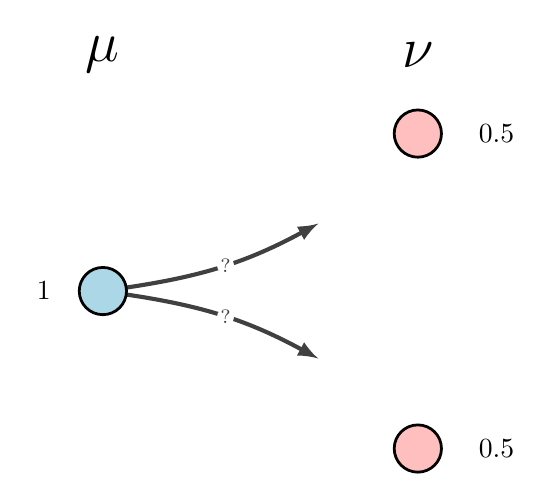
\begin{tikzpicture}
\Vertex[y=2,x=0]{A}
\Vertex[y=0,x=4,color=pink]{B}
\Vertex[y=4,x=4, color=pink]{C}
\Vertex[y=3,x=3, Pseudo, color=pink]{D}
\Vertex[y=1,x=3, Pseudo, color=pink]{E}

\Edge[Direct, label=?, bend=-10](A)(D)
\Edge[Direct, label=?, bend=10](A)(E)
\node[] at (0,5) {\huge$ \mathbf {\mu}$};
\node[] at (4,5) {\huge$ \mathbf {\nu}$};
\node[] at (5,0) {0.5};
\node[] at (5,4) {0.5};
\node[] at (-0.75,2) {1};

\end{tikzpicture}

\end{document}